
\section{Active Learning for \coref{} through Simulations and Humans}
\label{sec:experiments}

We run experiments to understand two important factors of active learning for
\coref{}: sources of model
uncertainty (Section~\ref{ssec:uncertainty}) and balancing reading against
labeling
(Sections~\ref{ssec:tradeoff}).
First, we simulate active learning on \preco{} to compare sampling strategies
based on various forms of uncertainty
(Section~\ref{ssec:sampling_results}).
Then, we set up a user study to investigate how humans perform when labeling
spans from fewer or more documents from \preco{} (Section~\ref{ssec:human_labeling}).
Specifically, we analyze their annotation time and throughput.
Finally, we run large-scale simulations on \preco{} and
\qbcoref{} (Section~\ref{ssec:adaptation}).
We explore different combinations of sampling strategies and labeling
configurations.

\paragraph{Models}
In all experiments, the source model is the best checkpoint of \icoref{} model
 trained on
\ontonotes{}~\citep{xia-2020}
with
\spanbertlarge~\citep{joshi-2020} encoder.
For continued training on the target dataset, we optimize with a fixed parameter
configuration (Appendix~\ref{ssec:params}).
We evaluate models on
\avgfone{}, the averaged \fone{} scores of \abr{muc}~\citep{vilain-1995}, $\abr{b}^3$~\citep{bagga-1998},
and $\abr{ceaf}_{\phi4}$~\citep{luo-2005}.
For all synthetic experiments, we simulate active learning with gold data
substituting as an annotator. However, gold mention boundaries are not used when
sampling data. The model scores spans that are likely to be entity
mentions for inference, so we limit the active learning candidates to this pool of high-scoring
spans.
For each active learning simulation, we repeat five runs with different random seed initializations.
\paragraph{Baselines}
We compare the proposed sampling strategies (Section~\ref{ssec:entropy})
along with \textbf{li-clust-ent}, which is
clustered entropy from \citet{li-2020} (Equation~\ref{eq:li-clust-ent}).
Active learning is frustratingly less effective than random sampling in many settings~\citep{lowell-2019}, so we include two random baselines in our
simulation. \textbf{Random} samples from all spans in the
documents. \textbf{Random-ment}, as well as other strategies, samples only from the
pool of likely (high-scoring) spans.
Thus, \textbf{random-ment} should be a stronger
baseline than \textbf{random}.

\begin{figure}[!t]
    \centering
    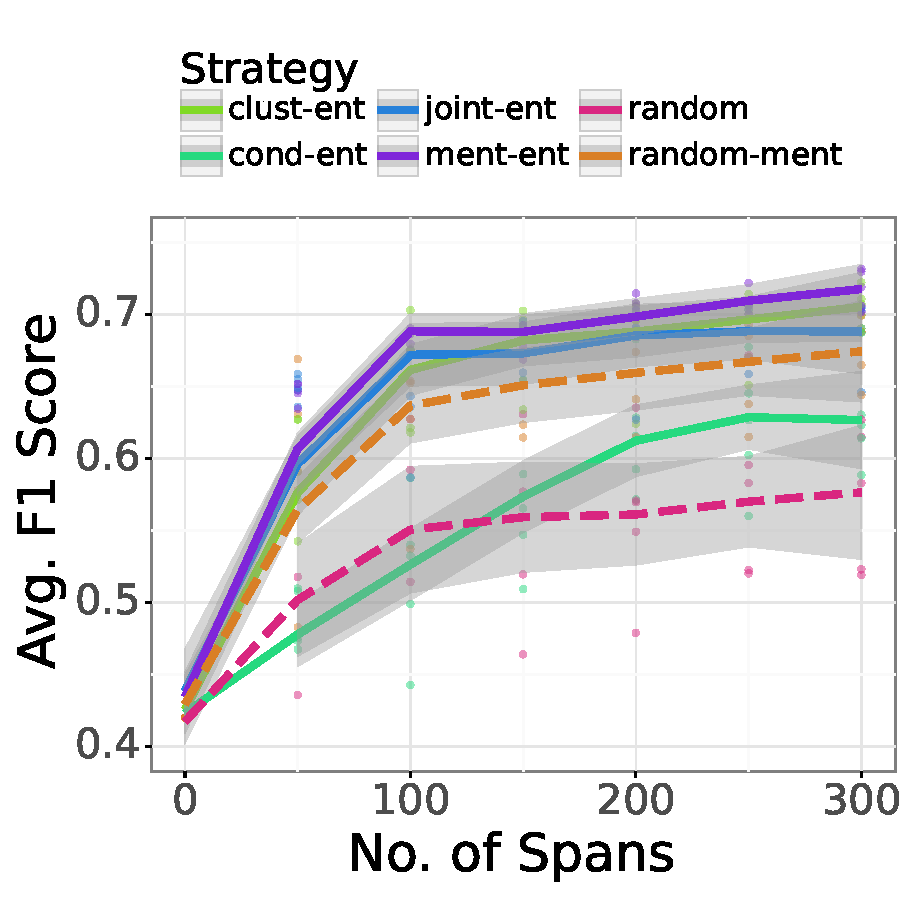
\includegraphics[width=\linewidth]{preco_simple_f1.pdf}
    \caption{Test \avgfone{} on \preco{} for each strategy.
    On each
    cycle,
    fifty spans from one document are sampled and labeled.
    We repeat each
    simulation five times.
    \textbf{Ment-ent},
    \textbf{clust-ent}, and \textbf{joint-ent} are most  effective
    while
    \textbf{random} hurts the model the most.
    }
    \label{fig:preco_simple}
\end{figure}

\begin{figure}[!t]
    \centering
    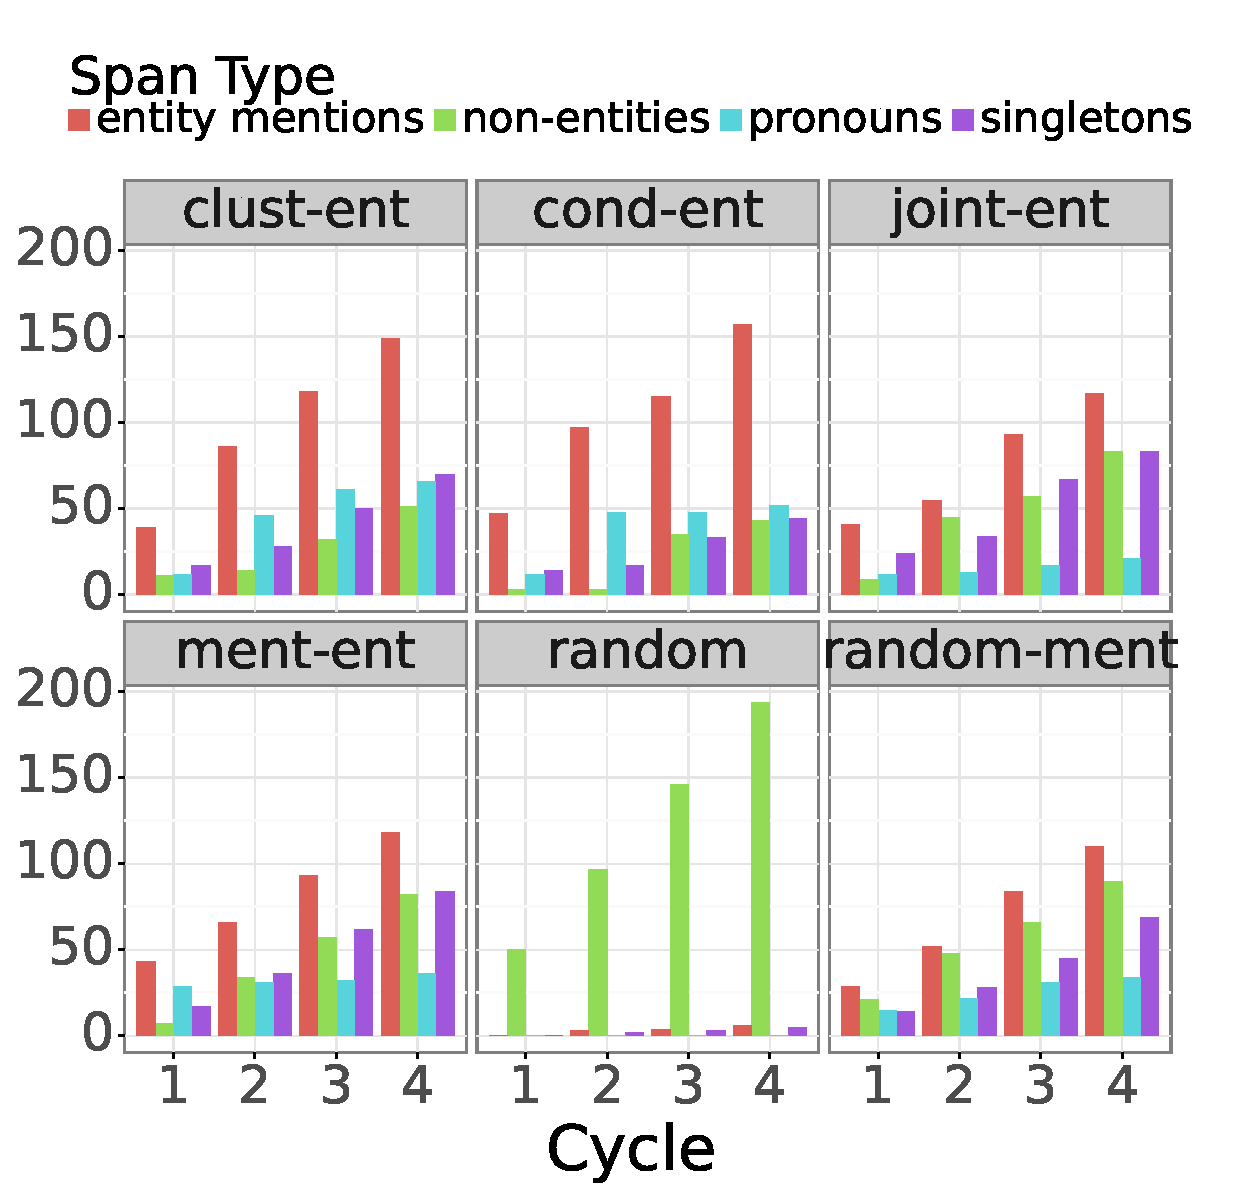
\includegraphics[width=\linewidth]{preco_samples.pdf}
    \caption{Cumulative counts of entities, non-entities, pronouns, and
    singletons
    sampled for each strategy over first four cycles of the \preco{} simulation. \textbf{Random} mostly samples
    non-entities. \textbf{Li-clust-ent} and \textbf{cond-ent} sample many
    entity mentions but avoid singletons.
    }
    \label{fig:preco_samples}
\end{figure}

\paragraph{Datasets}

\ontonotes~{\small 5.0} is the most common dataset for training and evaluating
\coref{}~\citep{pradhan-2013}.
The dataset contains news articles
and telephone conversations. Only non-singletons are annotated.
Our experiments transfer a model trained on \ontonotes{} to two
target datasets: \preco{} and \qbcoref{}.
\preco{} is a large corpus of grade-school reading comprehension
texts~\citep{chen-2018-preco}.
Unlike \ontonotes{}, \preco{} has annotated singletons. There are 37K training, 500 validation, and 500 test
documents.
Because the training set is so large, \citet{chen-2018-preco} only analyze
subsets of 2.5K documents.
Likewise, we reduce the training set to a subset of 2.5K
documents, comparable to the size of \ontonotes{}.

The \qbcoref{} dataset~\citep{guha-2015} contains trivia questions from Quizbowl
tournaments
that are densely packed with
entities from academic topics.
Like \preco{}, singletons are
annotated.
Unlike other datasets, the syntax is idiosyncratic and world knowledge is needed
to solve coreference.
Examples are pronouns before the first mention of named
entities and oblique references like ``this polity'' for
``the Hanseatic League''.
These complicated structures rarely occur in everyday text but serve
as challenging examples for \coref{}.
There are 240 training, 80
validation, and 80 test documents.



\subsection{Simulation: Uncertainty Sampling}
\label{ssec:sampling_results}

To compare different sampling
strategies, we first run experiments on \preco{}. We sample fifty spans from one document for each cycle. By the end
of a simulation run, 300 spans are sampled from six documents. For this
configuration, uncertainty sampling strategies generally reach higher accuracy
than the random baselines (Figure~\ref{fig:preco_simple}),
but \textbf{cond-ent} and \textbf{li-clust-ent} are worse than \textbf{random-ment}.

\subsubsection{Distribution of Sampled Span Types}
\label{ssec:distribution}
To understand the type of spans being sampled, we count entity
mentions,
non-entities, pronouns, and singletons that are sampled by each strategy
(Figure~\ref{fig:preco_samples}). \textbf{Random} samples very few
entities, while other strategies sample more entity mentions. \textbf{Clust-ent} and
\textbf{cond-ent} sample more entity mentions and pronouns because the sampling objective
prioritizes mentions that are difficult to link.
\textbf{Clust-ent}, \textbf{joint-ent}, and \textbf{ment-ent} sample more
singleton mentions. These strategies also show higher \avgfone{}
(Figure~\ref{fig:preco_simple}). For transferring from \ontonotes{} to \preco{},
annotating singletons is useful because only non-singleton mentions are labeled
in \ontonotes{}.  We notice \textbf{ment-ent} sampling pronouns, which
should obviously be entity mentions, only in the first cycle.
Many pronouns in \ontonotes{} are singletons, so the mention detector has trouble
distinguishing them initially in \preco{}.


\begin{figure}[!t]
    \centering
    \includegraphics[width=\linewidth]{preco_error.pdf}
    \caption{For each sampling strategy, we analyze the model from the last
    cycle of its \preco{} simulation. We compare the number of errors across common error
    types in \coref{}. The \textbf{source} \ontonotes{} model
    severely suffers from \emph{missing entities} and \emph{missing mentions}.
    \textbf{Ment-ent} helps most with reducing these errors.
    }
    \label{fig:preco_error}
\end{figure}


\subsubsection{Error Analysis}
\label{ssec:error}
\citet{kummerfeld-2013} enumerate the ways \coref{} models can go wrong:
\emph{missing entity}, \emph{extra entity}, \emph{missing mention}, \emph{extra
mention}, \emph{divided entity},
and \emph{conflated entity}. \emph{Missing entity} means a gold entity
cluster is missing. \emph{Missing mention} means a mention span for a gold
entity cluster is missing.  The same definitions apply for \emph{extra entity}
and \emph{extra mention}.
\emph{Divided entity} occurs when the model splits a gold entity cluster into
multiple ones. \emph{Conflated entity} happens when the model merges
gold entity clusters. For each strategy, we analyze the
errors of its final model from the
simulation's last cycle (Figure~\ref{fig:preco_error}).
We compare against the
\textbf{source} model that is only trained on \ontonotes{}.

The \textbf{source}
model makes many \emph{missing entity} and \emph{missing mention} errors.
It does not detect several entity spans in \preco{}, like
locations (``Long Island'') or ones spanning multiple words (``his kind
acts of providing everything that I needed'').
These spans are detected by uncertainty sampling strategies and \textbf{rand-ment}. \textbf{Ment-ent} is most effective at reducing ``missing''
errors. It detects gold entity clusters like
``constant communication'' and ``the best educated guess about the storm''.
By training on spans that confuse the mention detector, the model adapts to the
new domain by understanding what constitutes as an entity mention.

Surprisingly, \textbf{li-clust-ent} makes at least twice as many \emph{extra entity} and
\emph{extra mention}
errors than any other strategy. For the sentence, ``Living in a large building with only 10 bedrooms'', the
gold data identifies two entities: ``a large building with only 10
bedrooms'' and ``10 bedrooms''.
In both \ontonotes{} and \preco{}, the guidelines only allow the longest noun
phrase to be annotated.
Yet, the \textbf{li-clust-ent} model predicts additional mentions,
``a large building'' and ``only 10 bedrooms''.
We find that \textbf{li-clust-ent} tends to sample nested
spans (Table~\ref{tab:examples_preco}). Due to the summed entropy computation, nested spans
share similar values for clustered entropy as they share similar
antecedent-linking probabilities. This causes the \emph{extra entity} and
\emph{extra mention} errors because the model predicts there are additional
entity mentions within a mention span.


Finally, we see a stark difference between \textbf{random-ment} and \textbf{random}.
Out of all the sampling strategies, \textbf{random} is least effective at preventing \emph{missing entity} and \emph{missing mention} errors.
We are more likely to sample non-entities if we randomly sample from all spans in the document (Appendix~\ref{ssec:examples}).
By limiting the sampling pool to only spans that are likely to be entity mentions, we sample more spans that are useful to label for \coref{}.  Thus, the mention detector from neural models should be deployed during active learning.




\subsection{User Study: Reading and Labeling}
\label{ssec:human_labeling}


We hold a user study to observe the trade-off between reading and labeling.
Three annotators, with minimal \abr{nlp} knowledge, label spans
sampled from \preco{}. We use \textbf{ment-ent} to sample spans because the
strategy shows highest \avgfone{} (Figure~\ref{fig:preco_simple}).
First, the users read instructions (Appendix~\ref{ssec:user_appendix}) and practice labeling for
ten minutes.
Then, they complete two sessions: \textbf{FewDocs} and \textbf{ManyDocs}.
In each session, they label as much as possible for at least twenty-five
minutes.
In \textbf{FewDocs}, they read fewer documents and label roughly
seven spans per document.
In \textbf{ManyDocs}, they read more documents and label
about one span per document.

For labeling coreference, we develop a user interface that is open-sourced
(Figure~\ref{fig:ui}).
 To label the
 antecedent of
 the highlighted span, the user clicks on a contiguous span of tokens.
 The interface suggests
 overlapping candidates based on the spans that are retained by the \coref{}
 model.

In the user study, participants label at least twice as much
in \textbf{FewDocs} compared to \textbf{ManyDocs} (Figure~\ref{fig:user}).
By labeling more spans in \textbf{FewDocs}, the mean \avgfone{} score is also
slightly higher.
Our findings show that the number
of read documents should be constrained to increase labeling
throughput.
Difference in number of labeled spans between \textbf{FewDocs}
and \textbf{ManyDocs} is more pronounced when two annotators volunteer to continue labeling after required duration
(Appendix~\ref{ssec:user_appendix}).

\begin{figure}[!t]
\centering
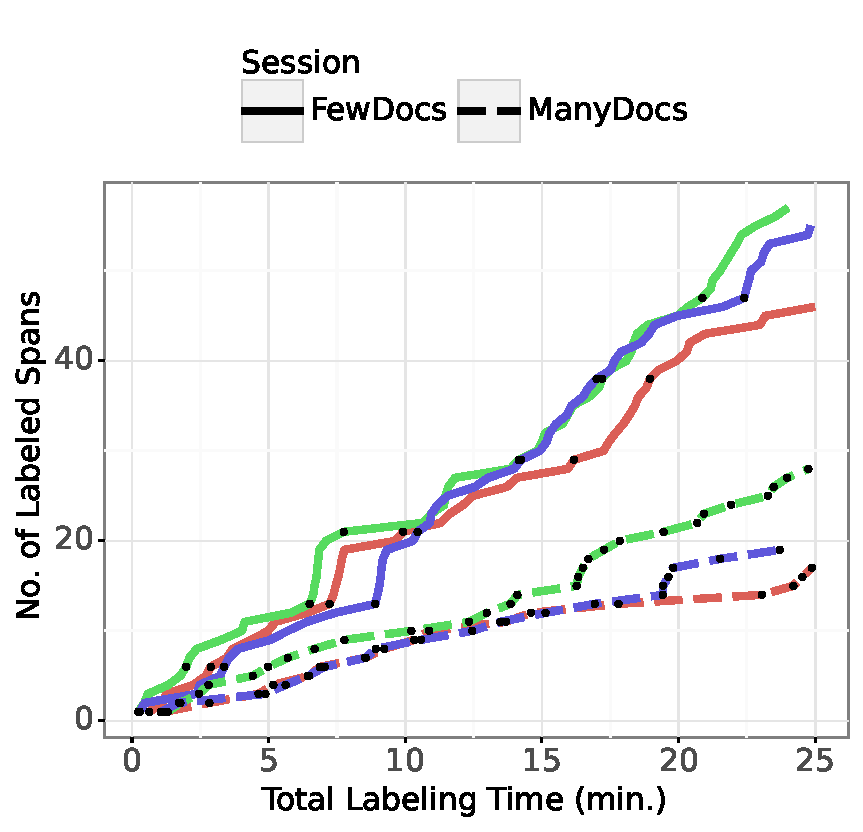
\includegraphics[width=\linewidth]{userstudy_reduced.pdf}
\caption{The number of spans labeled within twenty-five minutes.
Each color indicates one of three users and the linetype
    designates the session.
Black dots mark the first span labeled in a different
    document. The mean \avgfone{} across users for each session is
    on the right. By restricting the number of read documents in
    \textbf{FewDocs}, users label at least twice as many spans and the model
    slightly
    improves in \avgfone{}. }
\label{fig:user}
\end{figure}


\begin{figure}[!t]
    \centering
    \begin{subfigure}[t]{\linewidth}
        \centering
        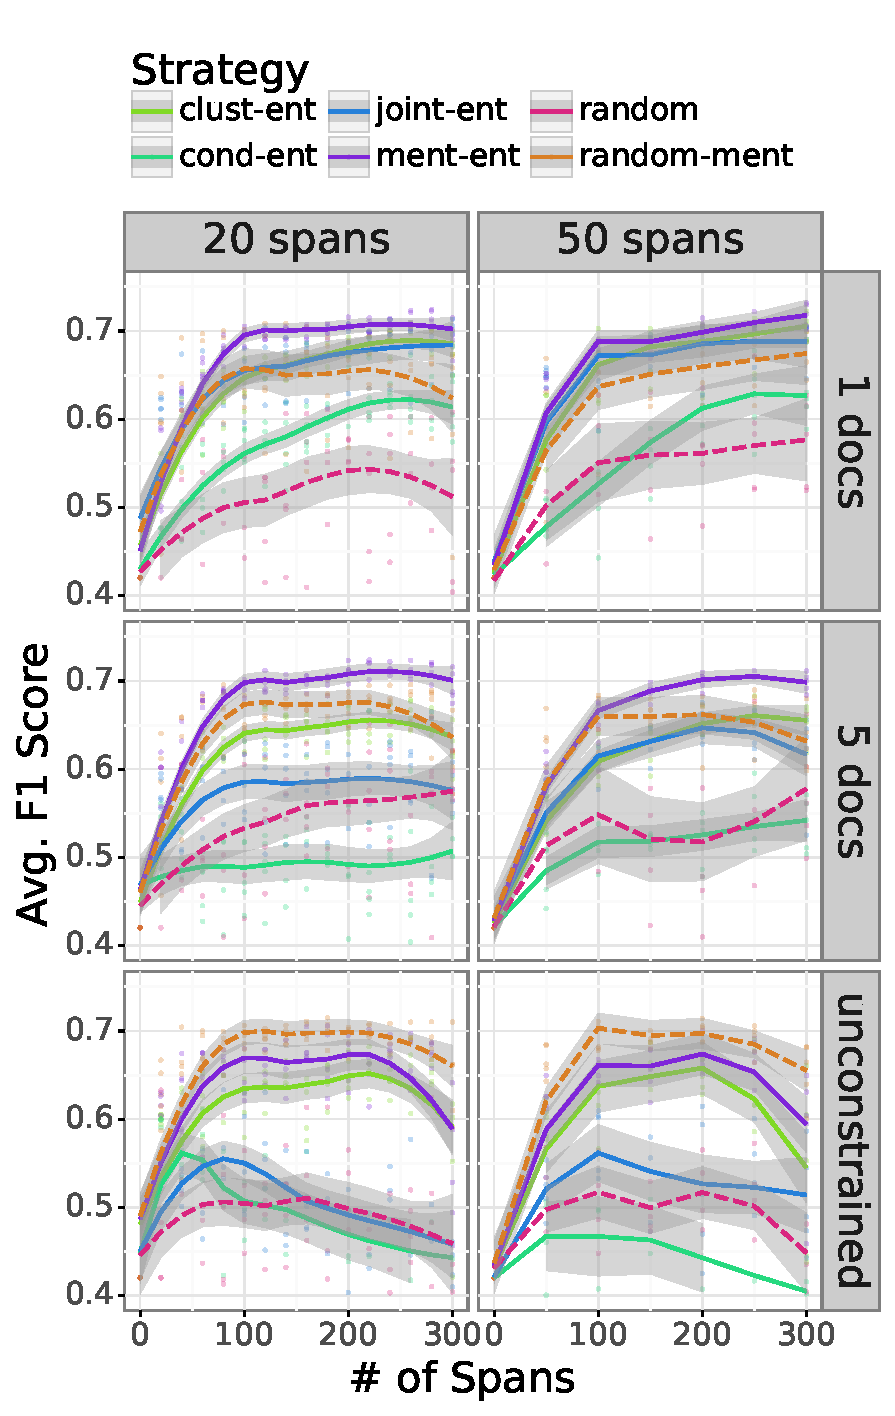
\includegraphics[width=0.90\linewidth]{preco_f1.pdf}
        \caption{\preco{}}
        \label{fig:preco}
    \end{subfigure}
    \begin{subfigure}[t]{\linewidth}
        \centering
        \includegraphics[width=0.80\linewidth]{qbcoref_f1.pdf}
        \caption{\qbcoref{}}
        \label{fig:qbcoref}
    \end{subfigure}
    \caption{Test \avgfone{} on \preco{} and \qbcoref{} of each strategy
    throughout simulations. Each row varies in~$m$, the maximum number of
    documents read per cycle. Each column varies in $k$, the number of annotated
    spans per cycle.
    For~$m$ of one or five, \textbf{ment-ent} shows highest \avgfone{}
    for \preco{} and other uncertainty sampling strategies are best for
    \qbcoref{}. When $m$ is unconstrained, many strategies show unstable
    training.
    }
    \label{fig:f1}
\end{figure}

\subsection{Simulation: Uncertainty Sampling and Reading-Labeling Trade-off}
\label{ssec:adaptation}

We finally run simulations to explore \textit{both} sources of model uncertainty and the
trade-off between reading and labeling. The earlier experiments have individually
looked at each aspect.
Now, we analyze the interaction between both factors to understand which
combination works best for adapting \coref{} to new domains.
We run simulations on \preco{} and \qbcoref{} that trade-off the number
of documents read~$m$ with the number of annotated spans~$k$
(Figure~\ref{fig:f1}).  We vary~$m$ between one, five, and an unconstrained number of documents.
For \preco{}, we set~$k$ to twenty and fifty.
For \qbcoref{}, we set~$k$ to twenty and forty.
These results are also presented in numerical form (Appendix~\ref{ssec:num}).

\paragraph{\preco{}}
For \preco{}, the test \avgfone{} of
\icoref{} trained on the full training dataset is 0.860.
When $m$ is constrained to one or five, \avgfone{} can reach around 0.707 from
training the model on only 300 spans sampled by
\textbf{ment-ent}.
As $m$ increases, fewer spans are sampled per document and
all sampling strategies deteriorate.
After training on sparsely annotated documents, the model tends to predict
singletons rather than cluster coreferent spans.
Like in the user study, we see
benefits when labeling more spans within a document.
Interestingly, \textbf{li-clust-ent} performs better when document
reading is not constrained to one document.
The issue with
\textbf{li-clust-ent} is that it samples nested mention spans
(Section~\ref{ssec:error}).
Duplicate sampling is less severe if spans can be sampled across more
documents. Another strategy that suffers from duplicate sampling is
\textbf{cond-ent} because it mainly samples pronouns. For some documents, the
pronouns all link to the same entity cluster.
As a result, the model trains on a
less diverse set of entity mentions and \textbf{cond-ent} drops in
\avgfone{} as the simulation continues.

\paragraph{\qbcoref{}}
For \qbcoref{}, the
test \avgfone{} of \icoref{} trained on the full training dataset is 0.795.
When we constrain $m$ to one or five, \textbf{li-clust-ent}, \textbf{clust-ent}, \textbf{cond-ent}, and
\textbf{joint-ent} have high \avgfone{}. Clustering entity mentions in
\qbcoref{} questions is difficult, so these strategies
help target ambiguous mentions (Table~\ref{tab:examples_qbcoref}). \textbf{Ment-ent} is less useful
because demonstratives are abundant in \qbcoref{} and
make mention detection easier.
\textbf{Li-clust-ent} still
samples nested entity mentions, but annotations for these spans help clarify
interwoven entities in Quizbowl questions. Unlike \preco{},
\textbf{li-clust-ent} does not sample duplicate entities because nested entity
mentions belong to different clusters and need to be distinguished.


Overall, the most helpful strategy depends on the domain.
For domains like
\preco{} that contain long documents with many singletons, \textbf{ment-ent} is
useful.
For domains like \qbcoref{} where resolving coreference is difficult,
we need to target linking uncertainty.
Regardless of the dataset,
\textbf{random} performs worst.
\textbf{Random-ment} has much higher \avgfone{}, which shows the importance
of the mention detector in active learning.
Future work should
determine the appropriate strategy for a given domain and annotation
setup.

